\documentclass[openany,11pt,a4paper]{report}

\usepackage{titlesec}
\titleformat{\chapter}
  {\normalfont\LARGE\bfseries}{\thechapter}{1em}{}
\titlespacing*{\chapter}{0pt}{-40pt}{10pt}

%{3.5ex plus 1ex minus .2ex}{2.3ex plus .2ex}

\usepackage{xcolor}
\usepackage{url}
\usepackage{array}
\usepackage{caption}
\usepackage{float}
%\usepackage{times}


\usepackage{amsmath} 
\usepackage{amssymb} 
\usepackage{bm}
\usepackage[colorlinks=true,breaklinks]{hyperref} 
\usepackage[hyphenbreaks]{breakurl} %
\usepackage{xcolor}
\definecolor{c1}{rgb}{0,0,1} % blue
\definecolor{c2}{rgb}{0,0.3,0.9} % light blue
\definecolor{c3}{rgb}{0.3,0,0.9} % red blue
\hypersetup{
linkcolor={c1}, 
citecolor={c2}, 
urlcolor={c3} 
}

\usepackage[nottoc]{tocbibind} 
\usepackage{graphicx}
\usepackage{longtable} 
\usepackage{bigstrut} 
\usepackage{enumerate}
\usepackage{todonotes} 
\usepackage{makeidx} 
\usepackage{color}


\usepackage{siunitx}
\usepackage{booktabs}




\usepackage{blindtext}


\makeindex

\usepackage[top=1.5cm, bottom=1.5cm,left=1.5cm,right=1.5cm]{geometry} % needed for page border settings
\parindent=0cm % for space of first line of new text block
\sloppy % for writing with hyphenless justification (tries to)
\hyphenation{} % use hyphenation of tolerance parameters, http://www.jr-x.de/publikationen/latex/tipps/zeilenumbruch.html
\hyphenpenalty=10000
\exhyphenpenalty=10000
\usepackage{fancyhdr}
%\usepackage[pdftex]{graphicx}
\usepackage{array,siunitx}
\usepackage{afterpage}





\begin{document}

\pagestyle{empty}


\begin{titlepage}

\newcommand{\HRule}{\rule{\linewidth}{0.5mm}} 
\center 

\textsc{\LARGE University of Cologne}\\[1.5cm]
\textsc{\Large Advanced Lab Course}\\[0.5cm] 

\vfill


\HRule \\[0.4cm]
{\huge \textbf {Experiment M2.3:
Transport properties of copper}}

 
\vfill

\begin{minipage}{0.4\textwidth}
\begin{flushleft} \large
\emph{Group 27}\\
Panagiota \textsc{Kardala}\\
Rabia \textsc{Zahid}
 
\end{flushleft}
\end{minipage}
~
\begin{minipage}{0.4\textwidth}
\begin{flushright} \large
\emph{Tutor:} \\
{Raphael German } 
\end{flushright}
\end{minipage}\\[4cm]


\vfill

{\large \today}\\[3cm] 

\vfill

\end{titlepage}



\pagestyle{plain}

\tableofcontents







\begin{abstract}
In this experiment we measure the Raman spectra of single crystalline samples in different polarization directions of the incoming and scattered
light, to obtain the Raman tensors of the observed excitations and determine their symmetries. determined. Moreover we explored the dependence of
the Raman spectrum on experimental parameters like the aperture width.


 First we fixed the alignment of the
spectrometer and then investigated the correlation of the width of the entrance slit with the line width by measuring a
rather sharp Raman line.v
\end{abstract}


\chapter{Theoretical background}

\section{Raman Spectroscopy}
There are various techniques to investigate the structure and composition of a crystal, for example X-ray diffraction (XRD) but it's not a fast measurement and the obtained diffraction pattern can easily be affected by impurities and Transmission electron microscopy (TEM) is destructive, time consuming and expensive. On the other hand Raman spectroscopy is a fast, non destructive technique that requires no sample preparation, with high spectral resolution. The use of Raman spectroscopy for predicting the crystal orientation is based on the intensity dependence of the Raman signal on the directions of the polarization vectors of the incident light relative to the crystallographic axes. The intensity of the Raman peaks depends on the lattice vibration, which is dependent on the polarization direction of the incident laser light and on the crystallographic grain orientations \cite{sos}. 


In the Raman
spectroscopy technique the structure and composition of the material are
probed. Specifically, when a photon
without enough energy to excite electronic transitions interacts with a molecule it can be scattered both elastically (Rayleigh scattering) and inelastically, where the latter is called Raman scattering and happens due to photons that couple to molecular vibrations or phonons in the
material. The inelastically  scattered photons can undergo energy loss (Stokes
scattering) or energy gain (anti-­Stokes
scattering).
The inelastic scattering of light with a molecule reveals its nature, since  each molecule has a specific set of vibrational bands defined by their
frequencies and intensities, that provide the formation about the local coordination of the atoms in the material \cite{1}. Roughly 1 in 10 million of photons are scattered inelastically and thus observe the Raman shift that expresses the frequency shift between the
incident laser light and the scattered light as


\begin{equation}
\qquad \Delta v\left(c m^{-1}\right)=v_{L}-v_{S}=\frac{10^{7}}{\lambda_{L}(n m)}-\frac{10^{7}}{\lambda_{R}(n m)}
\end{equation}

where $v_{S}$ and $v_{L}$ represents the absolute wave number of the scattered light and that of the laser.

\begin{figure}[H]
\centering
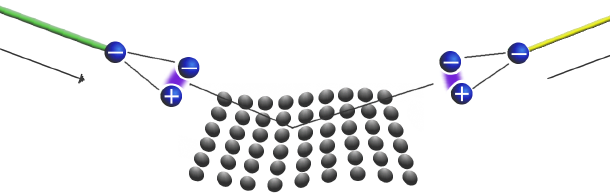
\includegraphics[scale=0.8]{solid.PNG}
\caption{\cite{phonons}}
\end{figure}



From the macroscopic point of view, an incoming photon is scattered at the lattice, inducing a phonon in the solid that reduces the energy of the photon by the energy lost in the scattering event. However, the direct interaction of the photon and the phonon is very improbable and non verified experimentally. The Raman process as it occurs in solid states involves the excitation of an electron from the incoming photon. The excited electron-hole pair is scattered and falls back to the origin state by
emission of a photon. Specifically, the Raman scattering event includes photon-electron and electron-lattice interaction. 


\cite{phonons}










Typically a Si Raman spectrum peak is located around $520 cm^{-1}$ depending on its
crystalline mass fraction, the asymmetric broadening of its width and the tail towards lower wave
numbers. Polarized Raman spectroscopy (PRS) is based on the
fact that the intensity of the Raman scattered light depends on the polarization of the incident laser
light relative to the crystal axes of the material being irradiated, so at a fixed sample position the change in the intensity of the scattered light is guided by the
symmetry selection rules of the sample and gives information concerning the sample crystal
orientation. \cite{sos}







The wavenumber in $cm^{-1}$ units corresponds to the inverse of the wavelength of a photon in vacuum, that has the same frequency as the measured phonon.










\section{PRS profiles}


A crystal structure is determined by the lattice and
the unit cell, which is repeated periodically with respect to the former, as illustrated bellow in Fig \ref{crystal}. \cite{W}


\begin{figure}[hbtp]
\centering
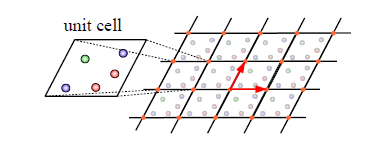
\includegraphics[scale=1]{Crystal.PNG}
\caption{\cite{W}}
\label{crystal}
\end{figure}

The Miller indices specify the directions and the plane of a lattice, where the number of indices matches the dimensions of the crystal, thus in a 3D crystal we have three Miller indices, as illustrated in Fig \ref{Miller}. 


\begin{figure}[H]
\centering
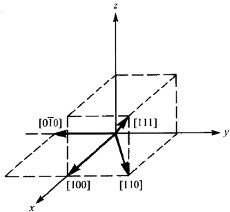
\includegraphics[scale=0.8]{Miller.jpg}
\caption{$[xyz]$ represents a direction. The negative directions are denoted with a bar on top of the
number. \cite{Si}}
\label{Miller}
\end{figure}



A vector $\mathbf{r}$ passing from the origin to a lattice point can be written as
 $\mathbf{r}=r_{1} \mathbf{a}+r_{2} \mathbf{b}+r_{3} \mathbf{c}$
where, $\mathbf{a}, \mathbf{b}, \mathbf{c}$ are the basic linearly independent lattice vectors and
 $\left(r_{1} r_{2} r_{3}\right)$ the Miller indices, thus $(xyz)$ represents a plane and $[xyz]$ the direction normal to the plane. Planes can involve multiple cells. \cite{Miller}\\

A primitive unit cell contains one lattice point and is invariant with respect to discrete translation by a translation vector $\mathbf{R}=n_{1} \mathbf{a}+n_{2} \mathbf{b}+n_{3} \mathbf{c}$
 











The crystal structure of Si is the Diamond structure, where its unit cell contains 8 atoms. For a $100 KeV/cm$ electric field, the rate of phonon emission has a maxima approximately at $66$ meV corresponding to $532$ $cm^{-1}$. \cite{energies}





\begin{figure}[H]
\centering
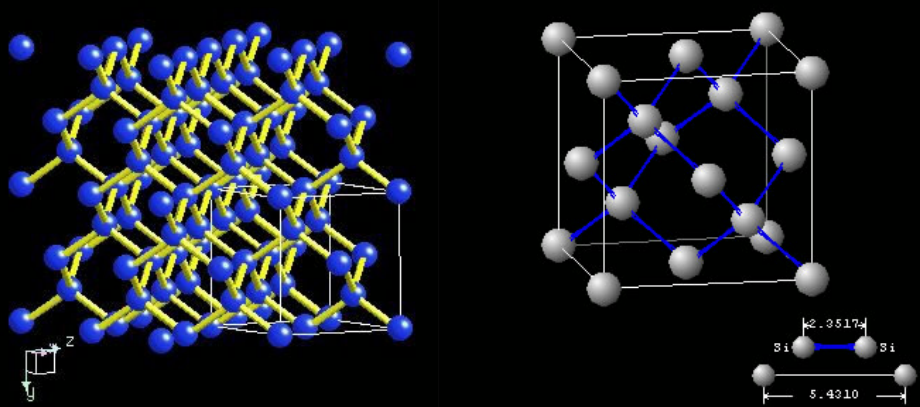
\includegraphics[scale=0.6]{diamondSi.PNG}
\caption{Si structure. \cite{Sipdf}}
\end{figure}



In this experiment we use Si crystal wafers of different symmetries, specifically  100 and 111. 




\begin{figure}[hbtp]
\centering
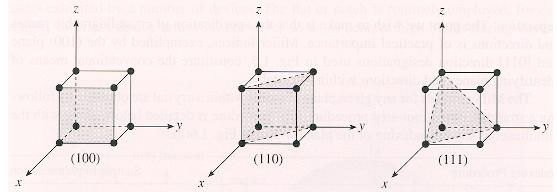
\includegraphics[scale=1.2]{Siorient.PNG}
\caption{Planes in different orientations of Si.}
\end{figure}




The amplitude of PRS profiles differs for different symmetry samples, it decreases as the number of intercepting axes in the Si wafers increases,
thus the (100) profile has the highest amplitude for varying polarization angle and the (111) has the
least.



According to Fig \ref{profiles}, the (100) maintains its four-fold symmetry since for the complete wafer rotation the PRS profile remains the same. The peak intensity variation as a function of rotation angle shows a consistent maxima and minima points at around 45 and 90 respectively.\\

The (111) shows two-fold rotational symmetry for each 180 rotation. The well known
3-fold rotation symmetry of the (111) wafer can be observed from the similar Raman
intensity value at 0 and 120 rotation. The (111) maintains its maxima and
minima positions for all rotations with much lower amplitude than both the (100).
This is a further indication that PRS profiles are unique depending on the crystallographic
structure of the irradiated samples.\\



\begin{figure}[H]
\centering
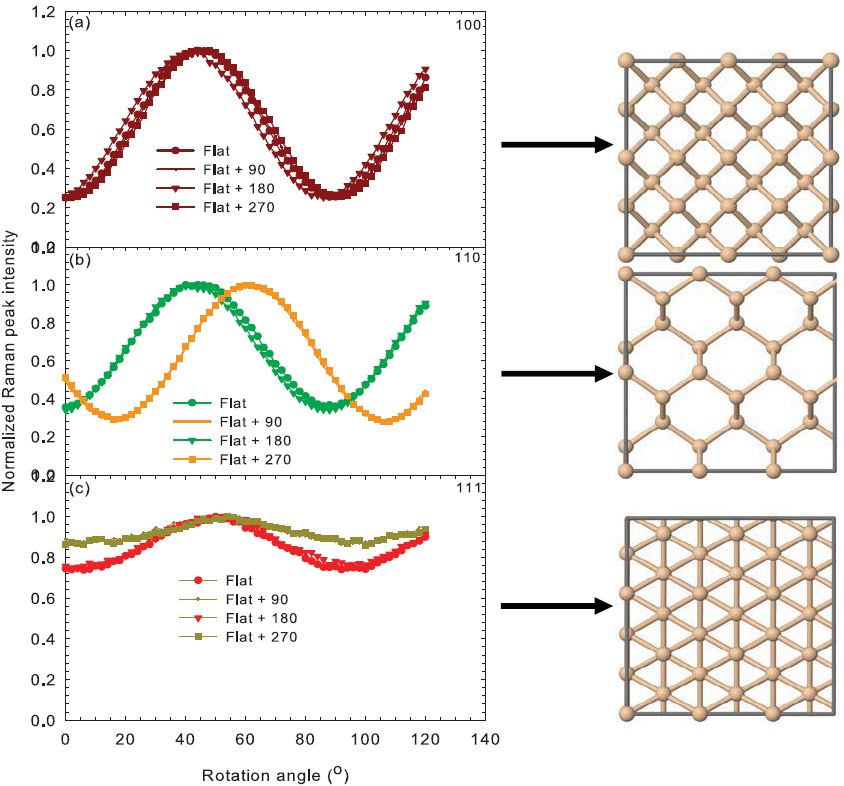
\includegraphics[scale=0.7]{Crystalsplots.PNG}
\caption{PRS profile of (100), (110) and (111) crystallic Si wafers. \cite{sos}}
\label{profiles}
\end{figure}








%Because our interest is in relating the Raman profile of the silicon wafers of known crystal orientation to the profile obtained in Si films we limited our comparison to measurements taken along the z-axis perpendicular to the primary flat because the primary flat has specific orientation relative to the wafer surface and is present in all the test wafers.

The variation in
rotation angle results in a change in the polarization plane of incident light and hence affects the Raman scattering intensity. We attribute this to the different degrees of scattering and energy
distribution within the crystal lattice of the silicon wafers depending on the crystal plane.\\



The $(111)$ plane has the largest number of silicon atoms per $cm^{2}$ whereas $(100)$ has the least. If the bond density in the
intercepting plane is high, will result in a more even distribution of the Raman intensity with
rotation angle, because more interactions between the plane and incident laser light are more likely to happen. The least dependence of Raman intensity on rotation angle is observed for the $(111)$ wafer, implying a more
even distribution of the scattered light, once it has more bonds within the lattice than the (100). Similarly, the (100) lattice has the least atomic bonds in its crystallographic
structure and thus scatters the least of the incident light. \cite{sos}





\begin{figure}[H]
\centering
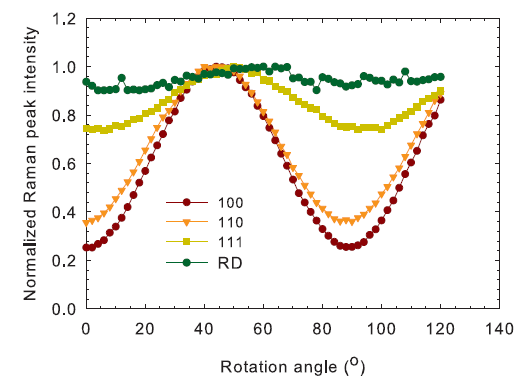
\includegraphics[scale=0.9]{Collective.PNG}
\caption{The Raman intensity at 520 $cm^{-1}$ as a function of rotation angle normalized to the
maximum intensity, for the three silicon wafers and silicon powder (RD). \cite{sos}}
\end{figure}



Since the frequency of the phonon Raman band depends on the
masses and positions of the atoms, the interatomic forces and the bond length, any effects altering those features will produce a change in the frequency of the band. The band position is sensitive to the presence of
stresses or strains because it increases the lattice spacing and thus decreases the wavenumber of the vibrational mode. On the other hand, the decrease of the lattice parameter yields an increase of the vibrational frequency. The sharp Lorentzian band
at $520 cm^{–1}$ of the first order Raman spectrum of crystalline silicon is quite sensitive to the presence of stress.\

Further, the presence of crystalline disorder also produces
changes in the frequency of the band, usually towards lower
wavenumbers. These are related to the breaking of translational symmetry in the crystal, which can be due to structural defects such as grain boundaries in nanocrystalline materials or dislocations. Raman bandwidth and bandshape are closely related to the crystalline order. In principle the bandwidth is related to the lifetime of the phonons. The presence of crystalline disorder produces a decrease of the phonon lifetime which thus generates an increase of the bandwidth. Therefore the density
of defects can be evaluated from the bandwidth. Damage in the lattice leads to a decrease of the intensity of the first
order modes, related to the breaking of bonds and changes
in atomic forces displacements, and hence produces a
decrease of the Raman polarizability tensors.
\cite{kiauto}

\newpage


\section{Lattice vibrations and Phonons}

\subsection{Phonons}

Starting from the very general concept of a ground state and the elementary excitations, we could describe the Bravais lattice and the phonons. The lattice potential has the shape of the Morse potential, arising from the valence electrons that are responsible for the lattice binding energy.

The harmonic approximation is used to describe the lattice excitations; in a vibrating lattice, the ground state electrons are attributed to the nucleus forming the ionic core, since the kinetic energy of the nucleus is $10^{4}$  times smaller than the one of the electrons, thus the electrons adjust instantly according to the nucleus position in an motional energy scale of eV while the lattice vibration is of the order of meV ($E_{ph}<100$ meV). In the treatment of the electron-phonon interaction, the nucleus kinetic potential is treated as a perturbation comparing to the electron Hamiltonian (Adiabatic approximation).
 The forces exerted between the atoms of neighbouring different cells, for maintaining their equilibrium position, are equal and dependant on their relative distance in a very simplifying relation to the "spring" constant, while the forces produced by distant atoms are effectively screened. 
 
 
Assuming longitudinal vibrations in a monochromatic cubic lattice (one atom is placed in every lattice point) along a high symmetry direction (i.e. all the distances in the plane remain constant) where all the atoms of the plane oscillate in phase, by symmetry the forces will be uniform and equal, acting in one direction only, resulting to an effective 1-D chain ($x$ direction) as illustrated in Fig \ref{1D}. \cite{CM1}
  
  
\begin{figure}[H]
\centering
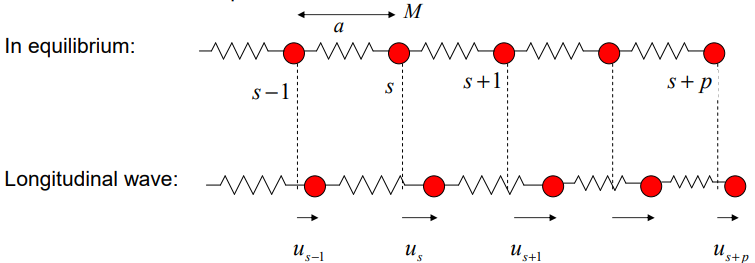
\includegraphics[scale=0.6]{1Dchain.PNG}
\caption{1-D chain of atoms. \cite{phonons}}
\label{1D}
\end{figure}
    

  
Solving the equation of motion for the harmonic potentials of the coupling of all the neighbouring atoms, we observe that the elastic response of the crystal is a linear function of the forces ( i.e.  the elastic energy is a quadratic function of the relative displacement), thus we obtain harmonic travelling waves of the form  
\begin{equation}
u_{s}= u e^{i(kx_{s}- \omega t)}
\end{equation}

where $x_{s}= s a$ is the position of the atom $s$ and $a$ the lattice constant (unit cell length  or the distance between atoms when the chain is in equilibrium). Proceeding through Newton' s 2nd law we obtain the dispersion relation of the crystal (illustrated in Fig \ref{1Ddispersion})
 
\begin{equation}
\omega (q)=2 \sqrt{\dfrac{C_{1}}{M}}  \mid sin (\dfrac{q a}{2}) \mid
\end{equation}
 
concerning the nearest neighbour ($C_{1}$),  where $- \dfrac{\pi}{a} \leq q  \leq \dfrac{\pi}{a} $ is the wave vector and $M$ the atom mass. \cite{phonons}\\
 
 
Now exploring the transverse vibrations in that lattice, we obtain equivalent effective 1-D chains along the $y$ and $z$ direction, but with different force constant between nearest-neighbour planes ($ C^{T}_{1} <   C^{L}_{1}  $), comparing to the longitudinal mode:
 
 
\begin{equation}
\begin{aligned}
\omega^{T} (\vec{q_{i}}) \neq  \omega ^{L} (\vec{q_{i}})  \\
 \omega^{T} (\vec{q_{i}}) =  \omega ^{T} (\vec{q_{j}}) \\
  \omega^{L} (\vec{q_{i}}) =  \omega ^{L} (\vec{q_{j}})
 \end{aligned}
\end{equation} 

where $\vec{q_{i}}= \vec{e_{x}},\vec{e_{y}},\vec{e_{z}}$. Usually the transverse modes have lower energy compared to the longitudinal and are often degenerate in high
symmetry directions.



\begin{figure}[H]
\centering
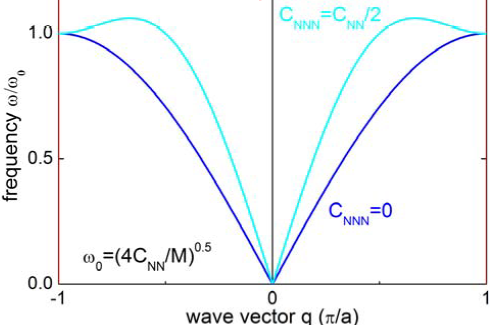
\includegraphics[scale=0.7]{phonon.PNG}
\caption{Harmonic frequency depending on the wavevector. $C_{NNN}=0$ corresponds to $C_{1}$ reffering to coupling with the first immediate neighbor, while for $C_{NNN}\neq 0$ the coupling to next immediate neighbor is included. \cite{CM1}}
\label{1Ddispersion}
\end{figure}




Concerning to the long wavelength limit $ \lambda \rightarrow \infty \Leftrightarrow  \omega (q=0)= 0  $, all the atoms move in the same phase, thus through the Goldstone theorem we can describe the massless excitations for $\lambda >> a  \Leftrightarrow q<< \frac{2 \pi}{a} $, called acoustic phonons because the sound velocity is given by $v_{s}= \omega /q$, where the dispersion relation is linear $\omega = cq$ and the discrete nature of the crystal lattice is irrelevant. The maximum energy of an acoustic phonon is roughly estimated at $ \hbar \omega _{a, max} \simeq 120 meV$.\\


For a 2-fold axes symmetry the degeneracy in the transverse modes is lifted and in general the dispersion is not isotropic, i.e. even the longitudinal modes in the planes $\vec{q} \parallel (100)$ and $\vec{q} \parallel (110)$ will be different.\\
 
 
Now if we consider two different mass atoms in a linear diatomic chain, the dispersion relation has two branches (Eq \ref{eq:branch}), separated by $\Delta \omega$, including thus the optical phonons, as illustrated in Fig \ref{1ddispersion}.


\begin{equation}
\omega^{2}(q)=C_{1}\left(\frac{M_{1}+M_{2}}{M_{1} M_{2}}\right) \pm
\sqrt{c_{1}^{2}\left(\frac{M_{1}+M_{2}}{M_{1} M_{2}}\right)^{2}-\frac{4 C_{1}^{2}}{M_{1} M_{2}} \sin ^{2}\left(\frac{qa}{2} \right)}
\label{eq:branch}
\end{equation}


\begin{figure}[H]
\centering
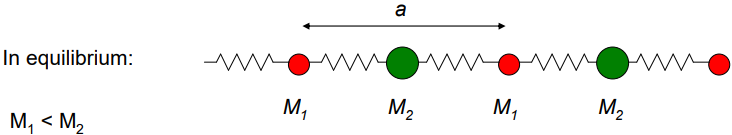
\includegraphics[scale=0.6]{2Dchain.PNG}
\caption{2D chain of atoms. \cite{phonons}}
\end{figure}




\begin{figure}[H]
\centering
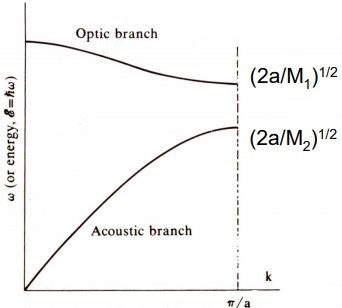
\includegraphics[scale=0.6]{2Ddispersion.jpg}
\caption{ $\omega $ vs $q$ for a linear diatomic 1-D chain, with $M1<M2$. \cite{phonons}}
\label{1ddispersion}
\end{figure}



Again the atoms oscillate in phase for $ \omega _{-} (q \rightarrow0)\rightarrow 0$ corresponding to the acoustic modes.\

On the other hand, for $\omega _{+} (q \rightarrow0)\rightarrow  \omega _{max}$ the atoms move exactly out of phase with amplitude ratio $\dfrac{M1}{M2}= -\dfrac{A2}{A1}$ and we obtain the so called optical phonons. An oscillating EM field could excite the optical modes if $M1$ and $M2$ have opposite charges, typically in the infrared region. For $q= \pm \frac{\pi}{a}$, at the zone boundary, we obtain standing waves for both modes, with $\omega _{-} (q=\frac{\pi}{a}) = \sqrt{\dfrac{2C}{M1}}$ and $\omega _{+}(q=\frac{\pi}{a}) = \sqrt{\dfrac{2C}{M}}$, where for $\omega _{-} $  $ M1$ is oscillating with $M2$ at rest and vice versa for $\omega _{+}$.

\begin{figure}[H]
\centering
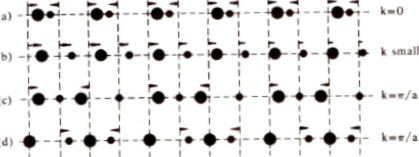
\includegraphics[scale=1.]{allmomentums.PNG}
\caption{
Schematic diagram showing the longitudinal atomic displacements for (a) $q=0$ optical branch, (b) acoustic branch for small $q$, (c) and (d) for the boundary zone modes for acoustic and oprical modes respectively.  \cite{phonons}}
\end{figure}





\begin{figure}[H]
\centering
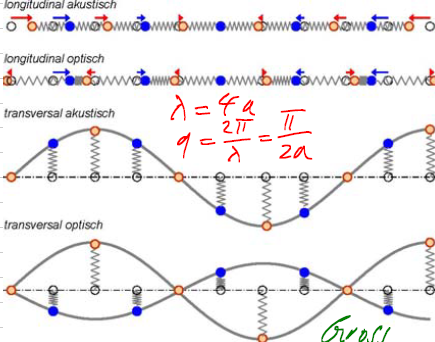
\includegraphics[scale=1]{allmomencp1.PNG}
\caption{Longitudinal and transverse oscillations for the acoustic and optical modes in the boundary zone condition, for $\lambda = 4a$. \cite{CM1}}
\end{figure}


The basic results of the $1D$ diatomic chain are valid for more complicated crystals as well. Asuming a basis of atoms $R$, we will have $3R$ branches in the dispersion relation where $3$ of them will be acoustic and the $3(R-1)$ optical.

\subsection{Quantization of phonons}

For high kinetic energy the lattice vibrations can be treated by classical harmonic oscillators, but for low energy the quantization is necessary. Assuming a bosonic field we extend the quantum harmonic oscillator to a $1D$ ring with $NN$ coupling as above, where we obtain a sum of independent oscillators that correspond to the phonons with quantized energy $E_{k}= \hbar \omega _{k}$, where $\omega^{2}_{k}= \dfrac{2C}{M} (1-cos(ka))$. Thus we can finally describe the phonons as the quantized excitations of the atomic/ionic displacement field of the lattice as quasi-particles, specifically bosons where their number is not conserved. Phonons interact with other quasi-particles as if they had a momentum  $ \hbar \vec{k}$, where a typical case of concern is scattering.










 by generalizing the 1D ring to a 3D crystal.1




\section{Raman Scattering}
When light of single frequency with a wavenumber $\bar{\nu_{0}}$ shines on a crystal, part of it transmits through the material and the rest is scattered away. In the elastic scattering the energy is conserved and there is no net momentum transfer in the crystal from the incoming particle, as it is distributed over all the atoms, so the phonon momentum remains the same. In the inelastic case though the energy in the crystal is transferred through the phonons, thus phonons can be created or annihilated (with finite lifetime), since the total momentum of the system has to be conserved. For an inelastic scattering experiment, the energy and momentum should be in the range of the phonons, thus $q \leq 1 A ^{-1}$ and $ \hbar \omega \leq 100 meV$. For the Brillouin zone center the requirement is $k \leqslant \frac{\pi}{a}$, i.e. $ \frac{qa}{\pi}\leq 10^{-3} $, thus the probing photons are either visible or infrared.

The conditions fulfilled must be 

\begin{equation}
\begin{aligned} k_{in} - k_{out}= q \simeq 0 \\ 
\hbar \Omega _{in} - \hbar \Omega _{out}= \pm \hbar \omega _{p} \end{aligned}
\end{equation}

Concerning to the outcoming frequency we obtain as illustrated in Fig \ref{stokes}  the different types of scaterring



\begin{equation}
\begin{aligned} 
\Omega _{out} =  \Omega _{in} - \omega _{p}  \; \; \; \; \; Stokes  \\ 
  \Omega _{out}= \Omega _{in} \; \; \; \; \; elastic  \;  Rayleigh  \; scattering  \\
 \Omega _{out}=  \Omega _{in} + \omega _{p} \; \; \; \; \; Anti- Stokes 
\end{aligned}
\end{equation}


\begin{figure}[H]
\centering
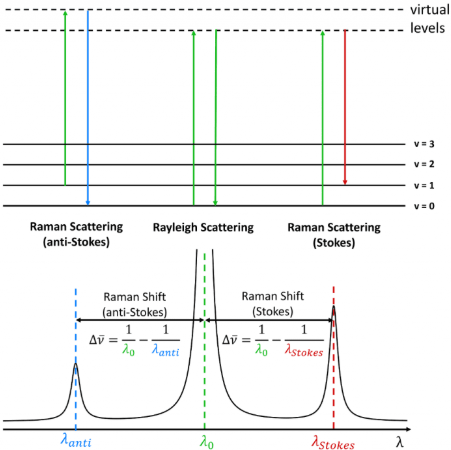
\includegraphics[scale=1.1]{stoke.PNG}
\caption{\cite{stokesdiagram}}
\label{stokes}
\end{figure}


\subsection{Classical Theory of inelastic Raman scattering}

Now taking under consideration the selection rules of the scattered light, that determine the intensity of the scattered light, the infrared active modes carry an electric dipole moment and the Raman active modes change the electrical polarizability.\\

In the classical theory interpretation, the inelastic light scattering is mediated by the scattering electronic polarizability of the medium, where the electromagnetic radiation theory can be used to explain the scattering phenomena. 

The dipole moment $\mu$ induced by the electric field is usually taken which is represented by power series. 
\begin{equation}
\mu=\mu^{(1)}+\mu^{(2)}+\mu^{(3)}+\cdots
\end{equation}

Where,

\begin{equation}
\begin{aligned} \mu^{(1)} &=\alpha \cdot \mathbf{E} \\ \mu^{(2)} &=\frac{1}{2} \beta \cdot \mathbf{E} \mathbf{E} \\ \mu^{(3)} &=\frac{1}{6} \gamma \cdot \mathbf{E} \mathbf{E} \mathbf{E} \end{aligned}
\end{equation}

Here, $\alpha$ is the polarizability tensor with magnitude 
$10^{-40} \mathrm{cv}^{-1} \mathrm{m}^{2}$, $\beta$ is $10^{-50} \mathrm{CV}^{-2} \mathrm{m}^{3}$ and $\gamma$ is $10^{-61} \mathrm{cv}^{-3} \mathrm{m}^{4}$. Rayleigh and Raman scattering are observed with low electric field intensities which is why it is usually explained by $\mu^{(1)}$ because $\mu^{(2)}$ and $\mu^{(3)}$ are very small for small electric field intensities.

The polarizability tensor for the interaction of a molecular system with the harmonically oscillating electric field is expressed by Taylor series,

\begin{equation}
\alpha_{i j}=\left(\alpha_{i j}\right)_{0}+\sum_{k}\left(\frac{\partial \alpha_{i j}}{\partial Q_{k}}\right)_{0} Q_{k}+\frac{1}{2} \sum_{k, l}\left(\frac{\partial^{2} \alpha_{i j}}{\partial Q_{k} \partial Q_{l}}\right)_{0} Q_{k} Q_{l}+\cdots
\end{equation}

Where, $\left(a_{i j}\right)_{0}$ is the $a_{i j}$ value at equilibrium and $Q_{k}$ and  $Q_{l}$ are normal coordinates. Now, for one normal mode,
\begin{equation}
\alpha_{i j}=\left(\alpha_{i j}\right)_{0}+\left(\frac{\partial \alpha_{i j}}{\partial Q_{k}}\right)_{0} Q_{k}
\end{equation}

For harmonic vibration,

\begin{equation}
Q_{k}=Q_{k 0} \cos \left(\omega_{k} t+\delta_{k}\right)
\end{equation}

Now, the induced dipole moment is,
\begin{equation}
\begin{array}{c}{\mu^{(1)}=\alpha_{k} \cdot \mathbf{E}_{0} \cos \omega_{0} t=\alpha_{0} \cdot \mathbf{E}_{0} \cos \omega_{0} t+\left(\frac{\partial \alpha_{k}}{\partial Q_{k}}\right)_{0} \cdot \mathbf{E}_{0} Q_{k 0} \cos \omega_{0} t \cos \left(\omega_{k} t+\delta_{k}\right) t=} \\ {\alpha_{0} \cdot \mathbf{E}_{0} \cos \omega_{0} t+\frac{1}{2}\left(\frac{\partial \alpha_{k}}{\partial Q_{k}}\right)_{0} \cdot \mathbf{E}_{0} Q_{k 0} \cos \left(\omega_{0} t+\omega_{k} t+\delta_{k}\right)+\frac{1}{2}\left(\frac{\partial \alpha_{k}}{\partial Q_{k}}\right)_{0} \cdot \mathbf{E}_{0} Q_{k 0} \cos \left(\omega_{0} t-\omega_{k} t-\delta_{k}\right)}\end{array}
\end{equation}

It can be seen that the dipole moment has three components of frequency.  Where, the first term is for Rayleigh scattering, the second for anti-stokes Raman scattering and the third is for Stokes Raman scattering. \cite{bib2}  


\subsection{Quantum Mechanical Theory}


Not every crystal lattice vibration can be probed by Raman scattering, there are certain selection rules that result form the energy and momentum conservation and are determined by the crystal symmetry and the symmetry of the excitations.






According to the quantum theory the emitted photon and the molecule can be considered as one system and the energy is transferred between them. 

The transition moment for such a system can be represented as,

\begin{equation}
\mathbf{M}_{f i}=\left\langle\Psi_{f}|\mu| \Psi_{i}\right\rangle
\end{equation} 

Where, $\psi_{i}$ and $\psi_{f}$ are the wave functions for the initial and final state and $\mu$ is the dipole moment operator. 

W know that classically,
\begin{equation}
\mu^{(1)}=\alpha \cdot \mathbf{E}
\end{equation}

Quantum mechanically,

$$
\mu_{f i}^{(1)}=\left\langle\Psi_{f}|\alpha| \Psi_{i}\right\rangle \cdot \mathbf{E}
$$

For Raman scattering, the typical matrix element of the polarizability tensor is, 



According to the quantum theory,

The total vibrational wavefunction becomes, 

\begin{equation}
\alpha_{x y}=\left(\alpha_{x y}\right){0}+\sum{k}\left(\frac{\partial \alpha_{x y}}{\partial Q_{k}}\right){0} Q{k}+\frac{1}{2} \sum_{k, l}\left(\frac{\partial^{2} \alpha_{i j}}{\partial Q_{k} \partial Q_{l}}\right){0} Q{k} Q_{l}+\cdots
\end{equation}

\begin{equation}
\left[\alpha_{x y}\right]{f i}=\left(\alpha{x y}\right){0}\left\langle\Phi{f} | \Phi_{i}\right\rangle+\sum_{k}\left(\frac{\partial \alpha_{x y}}{\partial Q_{k}}\right){0}\left\langle\Phi{f}\left|Q_{k}\right| \Phi_{i}\right\rangle
\end{equation}

\begin{equation}
\Phi_{i}=\prod_{k} \Phi_{v_{k}^{i}}\left(Q_{k}\right)
\end{equation}

\begin{equation}
\left\langle\Phi_{v_{k}^{\prime}}\left(Q_{k}\right) | \Phi_{v_{k}^{\prime}}\left(Q_{k}\right)\right\rangle=\left\{\begin{array}{l}{0 \text { for } v_{k}^{f} \neq v_{k}^{i}} \\ {1 \text { for } v_{k}^{f}=v_{k}^{i}}\end{array}\right.
\end{equation}


\begin{equation}
\left\langle\underset{v_{k}^{\prime}}{\left.\Phi_{v_{k}}^{\prime}\left(Q_{k}\right)\left|Q_{k}\right| \Phi_{v_{k}}\left(Q_{k}\right)\right\rangle}=\left\{\begin{array}{c}{0 \text { for } v_{k}^{f}=v_{k}^{i}} \\ {\left(v_{k}^{i}+1\right)^{\frac{1}{2}} b_{v_{k}} \text { for } v_{k}^{f}=v_{k}^{i}+1} \\ {\left(v_{k}^{i}\right)^{\frac{1}{2}} b_{v_{k}} \text { for } v_{k}^{f}=v_{k}^{i}-1}\end{array}\right.\right.
\end{equation}

\begin{equation}
b_{v_{k}}=\sqrt{\frac{h}{8 \pi^{2} v_{k}}}
\end{equation} 
\cite{bib2}





\subsection*{Raman activity and Raman tensor}
  

The geometry of the Raman experiment affects the Raman spectrum of a specific sample. The direction of the laser, the polarization of the laser light, the direction of the polarizer and the direction of the stray light which is analyzed by the spectrometer are  kept in mind for the specific crystallographic axes. These four parameters form the Porto notation. \\
The Raman tensor is a $3\times 3$  
tensor     
and its elements are related to the directions depends on the Porto noation b(ca)b. The Raman tensors shows if the phonon mode is Raman or not depending upon the symmetry. 
$$
\left(\begin{array}{lll}{a a} & {a b} & {a c} \\ {b a} & {b b} & {b c} \\ {c a} & {c b} & {c c}\end{array}\right)
$$
Figure 1.3 shows the back scattering geometry. 

\begin{figure}[H]
\centering
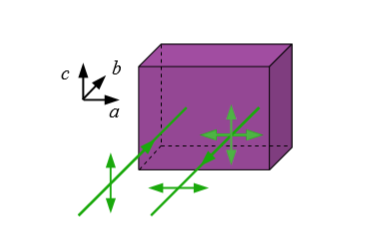
\includegraphics[scale=1]{geometry.PNG}    
\caption{}
\label{Fig:67}
\end{figure}

The following tensors are the example of a point group $$
C_{6 v}, A_{1}
$$ and $$
C_{2 v}, B_{1}
$$ symmetry.

$$
\left(\begin{array}{lll}{a} & {0} & {0} \\ {0} & {a} & {0} \\ {0} & {0} & {b}\end{array}\right) \quad\left(\begin{array}{lll}{0} & {0} & {f} \\ {0} & {0} & {0} \\ {g} & {0} & {0}\end{array}\right)
$$


Here, the zeros represent no phonon modes and the letters shows that the phonon modes are produced. It can be seen that the zeros are always symmetric. Whereas, the same letters represent that the phonon modes are degenerated. \cite{bib1}


\newpage

\section*{Our Raman tensors}

\begin{equation}
\mathcal{R}_{(100)}=\left(\begin{array}{ccc}{0} & {d} & {0} \\ {d} & {0} & {0} \\ {0} & {0} & {0}\end{array}\right)
\end{equation}




The intensity of the incoming laser light on the $(100)$ lattice is given as
\begin{equation}
I_{(100)} \propto\left|E_{o u t} \mathcal{R}_{(100)} E_{i n}\right|^{2}=d^{2} \sin ^{2}(2 \theta)
\end{equation}

while for the (111) lattice we obtain 

\begin{equation}
 I_{(111)} \simeq \left|E_{o u t} R^{-1} \mathcal{R}_{(100)} R E_{i n}\right|^{2}
\end{equation}


$R$ is the rotation matrix that rotates a vector along $(0,0,1)$ into a vector along
$(1,1,1)$ 

\begin{equation}
R=\left(\begin{array}{ccc}{\frac{1}{6}(\sqrt{3}-3)} & {\frac{1}{6}(\sqrt{3}+3)} & {\frac{1}{\sqrt{3}}} \\ {-\frac{1}{\sqrt{3}}} & {-\frac{1}{\sqrt{3}}} & {\frac{1}{\sqrt{3}}}\end{array}\right)
\end{equation}


hence we obtain the Raman tensor for the $(111)$ direction, as

\begin{equation}
\mathcal{R}_{(111)}=R^{-1} \mathcal{R}_{(100)} R=d\left(\begin{array}{ccc}{-1} & {0} & {0} \\ {0} & {-1} & {0} \\ {0} & {0} & {2}\end{array}\right)
\end{equation}

and finally the intensity of the outcoming light

\begin{equation}
I_{(111)} \simeq d^{2}
\end{equation}













\chapter{Experimental Setup}

In the beginning of the experiment we  aligned the spectrometer, where firstly we observed the dependence of the linewidth and the width of the entrance slit on the sharpness of the Raman line.\


Firstly we selected the alignment camera, switched on the monitor, open the entrance slit and removed the edge filter from the optical path in order to observe the laser spot. The sample surface was in the focus of the objective and the laser spot was focused on the sample as well as positioned in the center of the entrance slit. The spectrometer was moved to $0 cm^{-1}$ relative to the frequency of the laser in order to align the laser spot on the sample and the sample position, once the grating is acting as a mirror at this position. The spectrum was observed for a few seconds and then attenuators were removed in order to see the peak around $0 cm^{-1}$ to observe the laser spot.  To check the alignment, the edge filter and the attenuators were mounted again to block the laser light to protect the CCD camera and the spectrometer was moved at position $280 cm^{-1}$ relative to the laser line. Unfortunately, the wavelength was adjusted accordingly in order to see the peak at $521cm^{-1}$, but the peak center was shifted and we couldn't manage to obtain a better alignment, so we obtained the peak at $530cm^{-1}$ for Si (100) and $529cm^{-1}$ for Si (111). Afterwwards we measured the Si (111) and (100) surfaces, by zooming into the $530$ peak vicinity.\\

The Raman spectra of the samples were observed for all polarization directions. Specifically, the Raman spectra for two polarization direction (horizontal h / Vertical v) can be observed in combination with two polarizations of laser (h/v) which leads to four spectra hh, vv, hv and vh, where  the last two are equal. For the measurements under different polarization, the change in the light polarization is induced by the two mounted polarizers placed in front of the the laser and spectrometer. The laser light was incident perpendicularly on the sample surface along the z axis.


Further, we measured the spectrum for 10  different width of the
entrance slit.



\begin{figure}[hbtp]
\centering
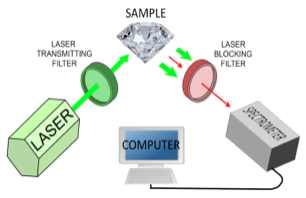
\includegraphics[scale=1.3]{setup.PNG}
\caption{A simple schematic representation of our experimental setup. \cite{setup}}
\end{figure}




\chapter{Analysis}

\section{Documentation of the spectrometer calibration}



Plot the spectrum obtained at the laser line and for the silicon 111 sample.
Fit the Si peak at 520  using a Lorentz profile and compare the values of
position and width of the peak to the literature.




\begin{figure}[H]
\centering
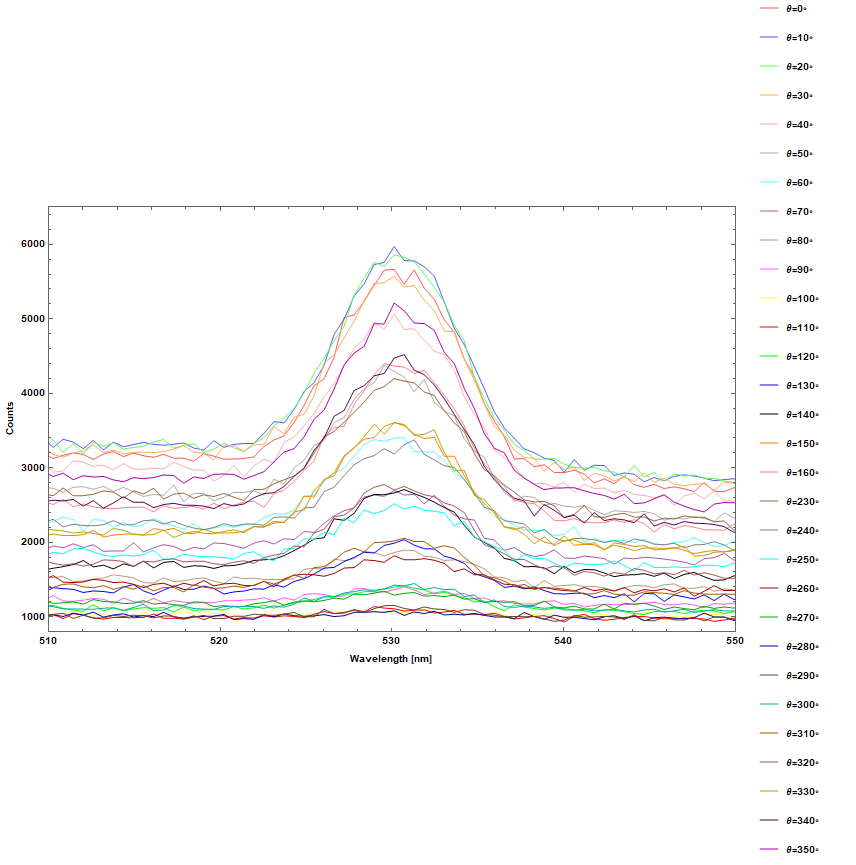
\includegraphics[scale=0.84]{100collectives.PNG}
\caption{100}
\end{figure}


\begin{figure}[H]
\centering
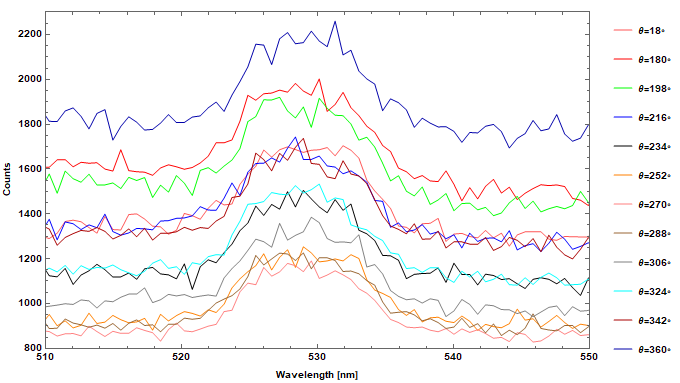
\includegraphics[scale=1]{111collectives.PNG}
\caption{111}
\end{figure}

\section{Determination of Raman tensors}

Plot for each sample the measured Raman spectra and determine the peak
position. Compare the peak positions of the different spectra (peaks of equal
frequency can be assigned to the same phonon mode). Establish the Raman
tensor for each phonon mode. A small contribution due to a slightly misaligned
polarizer or leakage of the polarizer must be neglected. Determine the symmetry
of the Phonon mode on basis of the Raman tensor.

\begin{figure}[H]
\centering
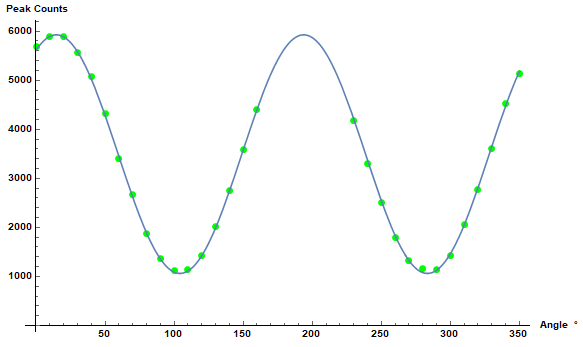
\includegraphics[scale=1]{100peaks.PNG}
\caption{100}
\end{figure}



\begin{figure}[H]
\centering
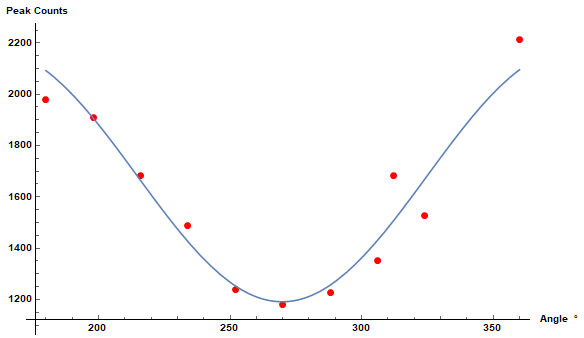
\includegraphics[scale=1]{111peaks.PNG}
\caption{111}
\end{figure}



\begin{figure}[H]
\centering
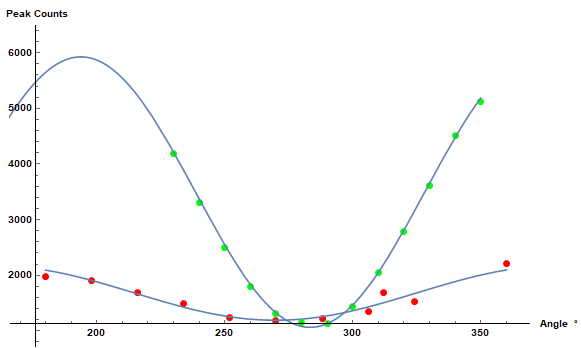
\includegraphics[scale=1]{collectivepeaks.PNG}
\caption{•}
\end{figure}




\section{Resolution of the spectrometer}


\begin{thebibliography}{99}


\bibitem{1} \url{http://physics.gu.se/~starn/tif060/Raman/Raman_manual2014.pdf}



\bibitem{W} Practical course M
Supplement: The Wurtzite Structure, Reinhard Rückamp, August 31, 2012


\bibitem{Si} \url{https://www.microchemicals.com/technical_information/silicon_crystallography.pdf}



\bibitem{Miller} \url{https://web.iit.edu/sites/web/files/departments/academic-affairs/academic-resource-center/pdfs/Miller_Indices.pdf}


\bibitem{setup} \url{https://agta.org/advantages-and-disadvantages-of-raman-fourier-transform-infrared-spectroscopy-ftir-in-the-gemological-field/}



\bibitem{phonons} \url{https://www.physik.fu-berlin.de/studium/praktika/fpa_dipl-ws2009/docs/Ma7_Raman.pdf}

\bibitem{energies} \url{https://www.researchgate.net/publication/227764230_Emission_and_absorption_of_phonons_in_silicon}

\bibitem{Sipdf} \url{https://www1.columbia.edu/sec/itc/ee/test2/pdf%20files/silicon%20basics.pdf}


\bibitem{} \url{https://onlinelibrary.wiley.com/doi/abs/10.1002/0471266965.com060.pub2}


\bibitem{sos} \url{http://www.chalcogen.ro/1461_Agbo.pdf}


\bibitem{kiauto} \url{https://analusis.edpsciences.org/articles/analusis/pdf/2000/01/jawhari.pdf}


\bibitem{phonons} \url{http://www.physics.uwo.ca/~lgonchar/courses/p9812/Lecture7_Phonons.pdf}


\bibitem{CM1} Condensed matter 1 lectures notes of prof Lorentz


\bibitem{stokesdiagram} \url{https://www.edinst.com/blog/what-is-the-stokes-shift/}

\end{thebibliography}






\end{document}
